\documentclass[aspectratio=169,10pt]{beamer}
\usepackage[T1]{fontenc}
\usepackage{amsmath,amssymb,amsfonts}
\usepackage{bm}
\usepackage{tikz}
\usepackage{xcolor}
\usetikzlibrary{arrows.meta,positioning,shapes,calc}

\definecolor{parchment}{HTML}{F4E8C8}
\definecolor{paper}{HTML}{FAF1D8}
\definecolor{ink}{HTML}{1A1A1A}
\definecolor{inkgray}{HTML}{5A5A5A}
\definecolor{accentred}{HTML}{8B1A1A}
\definecolor{accentgreen}{HTML}{2D5F2C}
\definecolor{accentblue}{HTML}{1F4E79}
\definecolor{redbg}{HTML}{F7E0DE}
\definecolor{grnbg}{HTML}{E0EBDC}
\definecolor{blubg}{HTML}{DDE6EF}
\definecolor{labelbg}{HTML}{EFE0B0}

\usefonttheme{serif}
\setbeamercolor{background canvas}{bg=parchment}
\setbeamercolor{normal text}{fg=ink}
\setbeamercolor{structure}{fg=ink}
\setbeamercolor{frametitle}{fg=ink,bg=parchment}
\setbeamercolor{title}{fg=ink}
\setbeamercolor{itemize item}{fg=ink}
\setbeamercolor{itemize subitem}{fg=ink}
\setbeamercolor{item}{fg=ink}
\setbeamercolor{caption name}{fg=ink}
\setbeamertemplate{navigation symbols}{}
\setbeamertemplate{itemize item}{\textbullet}

\setbeamertemplate{frametitle}{%
  \vspace{0.30em}%
  \begin{center}%
    {\bfseries\Large\insertframetitle\par}%
    \vspace{0.28em}%
    {\color{ink}\rule{0.86\paperwidth}{0.4pt}}%
  \end{center}%
  \vspace{0.10em}%
}
\setbeamertemplate{footline}{%
  \hbox to \paperwidth{\hfil\itshape\small\insertframenumber\hspace{0.7em}}%
  \vspace{0.35em}%
}

\newcommand{\vY}{\bm{Y}}
\newcommand{\vy}{\bm{y}}
\newcommand{\vA}{\bm{A}}
\newcommand{\vB}{\bm{B}}
\newcommand{\valpha}{\bm{\alpha}}
\newcommand{\vn}{\bm{n}}
\newcommand{\vs}{\bm{s}}
\newcommand{\vW}{\bm{W}}
\newcommand{\T}{^{\mathsf T}}
\newcommand{\Hh}{^{\mathsf H}}
\newcommand{\norm}[1]{\left\lVert #1\right\rVert}
\DeclareMathOperator*{\argmin}{arg\,min}

\tikzset{
  flowbox/.style={draw=ink,fill=paper,line width=0.6pt,
                  minimum width=2.5cm,minimum height=1.0cm,
                  align=center,font=\small\bfseries,inner sep=4pt},
  smallbox/.style={draw=ink,fill=paper,line width=0.4pt,
                   minimum width=0.7cm,minimum height=0.55cm,
                   inner sep=2pt,align=center,font=\footnotesize\itshape},
  method/.style={draw=accentgreen,fill=grnbg,line width=1.0pt,
                 align=center,font=\small\bfseries,inner sep=6pt},
  issue/.style={draw=accentred,fill=redbg,line width=1.0pt,
                align=center,font=\small\bfseries,inner sep=6pt},
  idea/.style={draw=accentblue,fill=blubg,line width=1.0pt,
               align=center,font=\small\bfseries,inner sep=6pt},
  flowarr/.style={-{Stealth[length=2.5mm,width=2mm]},line width=0.7pt},
  softarr/.style={-{Stealth[length=2mm,width=1.6mm]},line width=0.5pt,color=inkgray}
}

\newcommand{\bottomnote}[1]{%
  \begin{center}{\itshape\small #1}\end{center}}

\newcommand{\papercover}[4]{%
  \begin{frame}[plain]
    \vfill
    \begin{center}
      {\bfseries\Huge #1\par}
      \vspace{0.8cm}
      {\Large #2\par}
      \vspace{0.35cm}
      {\itshape\large\color{inkgray}#3\par}
      \vspace{0.55cm}
      {\small\texttt{\detokenize{#4}}\par}
    \end{center}
    \vfill
  \end{frame}}

\newcommand{\twocolmodel}[4]{%
  \begin{columns}[T,onlytextwidth]
    \begin{column}{0.48\textwidth}#1\end{column}
    \begin{column}{0.48\textwidth}#2\end{column}
  \end{columns}
  \bottomnote{#3\\#4}}


\usetikzlibrary{decorations.pathreplacing,decorations.pathmorphing,shapes.misc}

\newcommand{\jj}{\mathrm{j}}
\newcommand{\rx}{\mathrm{rx}}
\newcommand{\tx}{\mathrm{tx}}
\newcommand{\sinc}{\operatorname{sinc}}

\tikzset{
  stepbadge/.style={
    draw=ink, fill=labelbg, line width=0.6pt, circle,
    inner sep=0pt, minimum size=0.85cm,
    font=\bfseries\small
  },
  notecard/.style={
    draw=ink, fill=paper, line width=0.5pt, rounded corners=2pt,
    align=center, inner sep=5pt, font=\small
  },
  greencard/.style={
    draw=accentgreen, fill=grnbg, line width=0.8pt, rounded corners=2pt,
    align=center, inner sep=5pt, font=\small
  },
  redcard/.style={
    draw=accentred, fill=redbg, line width=0.8pt, rounded corners=2pt,
    align=center, inner sep=5pt, font=\small
  },
  bluecard/.style={
    draw=accentblue, fill=blubg, line width=0.8pt, rounded corners=2pt,
    align=center, inner sep=5pt, font=\small
  },
  brace/.style={decorate, decoration={brace, amplitude=4pt, raise=2pt}, line width=0.55pt, color=inkgray}
}

\newcommand{\storybadge}[2]{%
  \begin{tikzpicture}[remember picture,overlay]
    \node[stepbadge,anchor=north west,minimum size=0.62cm,font=\bfseries\footnotesize]
      at ([xshift=0.30cm,yshift=-1.62cm]current page.north west) {#1};
    \node[anchor=west,font=\scriptsize\itshape\color{inkgray}]
      at ([xshift=1.00cm,yshift=-1.92cm]current page.north west) {#2};
  \end{tikzpicture}%
}

\newcommand{\takeaway}[1]{\bottomnote{\textbf{Takeaway.} #1}}

\begin{document}

% =====================================================================
\begin{frame}[plain]
  \vspace{0.55cm}
  \begin{center}
    {\bfseries\Huge Doppler, ICI \& Partial FFT\par}
    \vspace{0.18cm}
    {\Large\itshape A grad-student version: one loop story, slowly\par}
    \vspace{0.40cm}
    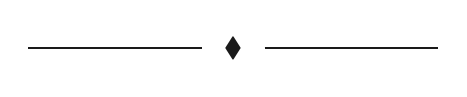
\begin{tikzpicture}
      \draw[ink,line width=0.5pt] (-2.6,0) -- (-0.4,0);
      \node at (0,0) {\color{ink}$\blacklozenge$};
      \draw[ink,line width=0.5pt] (0.4,0) -- (2.6,0);
    \end{tikzpicture}
    \vspace{0.35cm}

    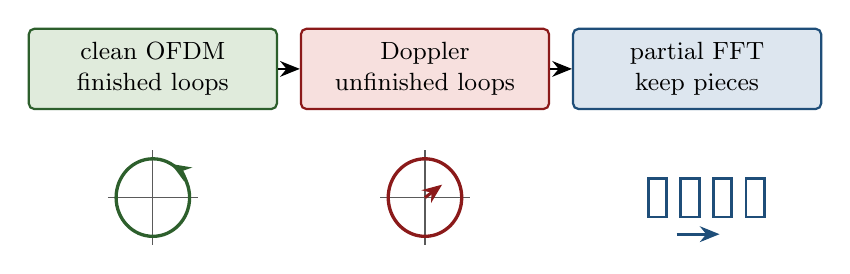
\begin{tikzpicture}[x=0.72cm,y=0.76cm,>=Latex]
      \node[greencard,text width=2.8cm] (a) at (-4.8,0.4) {clean OFDM\\finished loops};
      \node[redcard,text width=2.8cm] (b) at (0,0.4) {Doppler\\unfinished loops};
      \node[bluecard,text width=2.8cm] (c) at (4.8,0.4) {partial FFT\\keep pieces};
      \draw[flowarr] (a) -- (b);
      \draw[flowarr] (b) -- (c);

      \begin{scope}[shift={(-4.8,-1.75)},scale=0.72]
        \draw[inkgray] (-1.1,0)--(1.1,0);
        \draw[inkgray] (0,-1.1)--(0,1.1);
        \draw[accentgreen,line width=1.2pt] (0,0) circle (0.9);
        \draw[flowarr,color=accentgreen] (0.9,0) arc (0:60:0.9);
      \end{scope}
      \begin{scope}[shift={(0,-1.75)},scale=0.72]
        \draw[inkgray] (-1.1,0)--(1.1,0);
        \draw[inkgray] (0,-1.1)--(0,1.1);
        \draw[accentred,line width=1.2pt,domain=0:444,samples=100]
          plot ({0.9*cos(\x)},{0.9*sin(\x)});
        \draw[flowarr,color=accentred,line width=1.1pt] (0,0)--(0.42,0.30);
      \end{scope}
      \begin{scope}[shift={(4.8,-1.75)},scale=0.72]
        \foreach \x in {-1.2,-0.4,0.4,1.2} {
          \draw[accentblue,line width=1.0pt] (\x,-0.45) rectangle ++(0.45,0.9);
        }
        \draw[flowarr,color=accentblue,line width=1.0pt] (-0.5,-0.85)--(0.55,-0.85);
      \end{scope}
    \end{tikzpicture}
  \end{center}
\end{frame}

% =====================================================================
\begin{frame}{How to read this version}
\storybadge{0}{the map before the math}
\small
\begin{columns}[T,onlytextwidth]
  \begin{column}{0.48\textwidth}
    This deck answers four questions in order:
    \begin{enumerate}\setlength{\itemsep}{0.35em}
      \item What does the IFFT transmit?
      \item What does one FFT bin actually do?
      \item Why does Doppler make another carrier leak into my bin?
      \item Why does splitting the FFT into pieces help?
    \end{enumerate}
  \end{column}
  \begin{column}{0.48\textwidth}
    We use one running example:
    \[
      N=8,\qquad k=4,\qquad \ell=5.
    \]
    Bin $4$ is the receiver bin we inspect. Carrier $5$ is the neighbour that should cancel in clean OFDM.
    \vspace{0.15cm}
    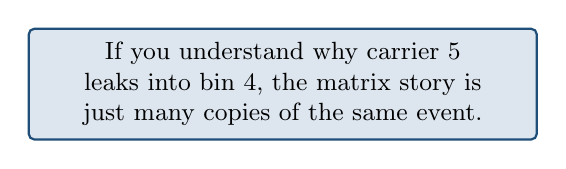
\begin{tikzpicture}
      \node[bluecard,text width=6.1cm] {%
        If you understand why carrier $5$ leaks into bin $4$, the matrix story is just many copies of the same event.};
    \end{tikzpicture}
  \end{column}
\end{columns}
\takeaway{One bin plus one neighbour is enough to understand ICI.}
\end{frame}

% =====================================================================
\begin{frame}{Vocabulary lock-in}
\storybadge{0}{one symbol, five names}
\small
\begin{center}
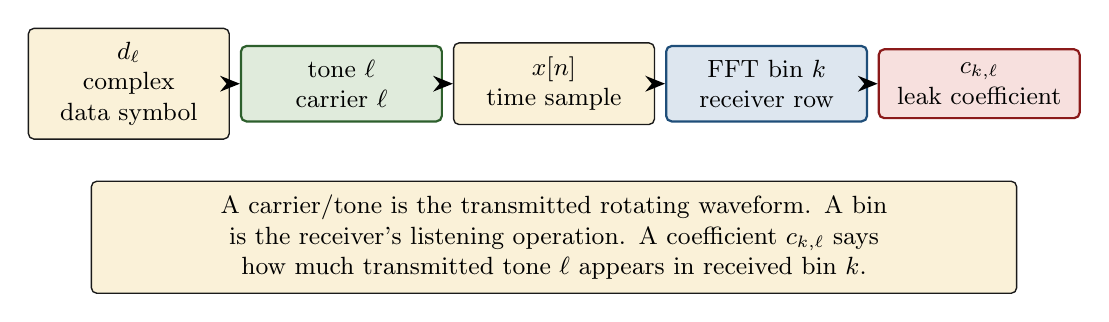
\begin{tikzpicture}[x=1cm,y=1cm,>=Latex]
  \node[notecard,text width=2.2cm] (d) at (-4.8,1.2) {$d_\ell$\\complex data symbol};
  \node[greencard,text width=2.2cm] (tone) at (-2.1,1.2) {tone $\ell$\\carrier $\ell$};
  \node[notecard,text width=2.2cm] (x) at (0.6,1.2) {$x[n]$\\time sample};
  \node[bluecard,text width=2.2cm] (bin) at (3.3,1.2) {FFT bin $k$\\receiver row};
  \node[redcard,text width=2.2cm] (c) at (6.0,1.2) {$c_{k,\ell}$\\leak coefficient};
  \draw[flowarr] (d) -- (tone);
  \draw[flowarr] (tone) -- (x);
  \draw[flowarr] (x) -- (bin);
  \draw[flowarr] (bin) -- (c);

  \node[notecard,text width=11.4cm] at (0.6,-0.75) {%
    A carrier/tone is the transmitted rotating waveform. A bin is the receiver's listening operation.
    A coefficient $c_{k,\ell}$ says how much transmitted tone $\ell$ appears in received bin $k$.};
\end{tikzpicture}
\end{center}
\takeaway{Carrier $\ell$ and bin $k$ are different roles; ICI happens when $\ell\ne k$ still leaves $c_{k,\ell}\ne0$.}
\end{frame}

% =====================================================================
\begin{frame}{The one-symbol OFDM chain}
\storybadge{1}{bits become clocks, then bins listen}
\small
\begin{center}
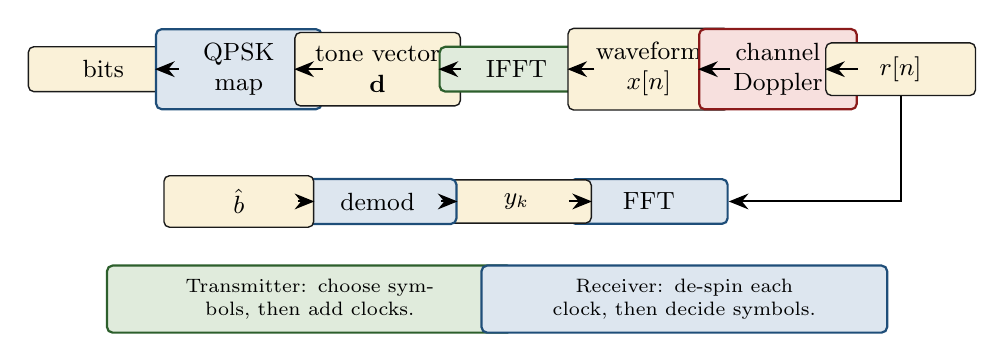
\begin{tikzpicture}[x=0.82cm,y=0.80cm,>=Latex]
  \node[notecard,text width=1.55cm] (bits) at (-6.2,1.0) {bits};
  \node[bluecard,text width=1.75cm] (qam) at (-4.10,1.0) {QPSK\\map};
  \node[notecard,text width=1.75cm] (d) at (-1.95,1.0) {tone vector\\$\mathbf d$};
  \node[greencard,text width=1.60cm] (ifft) at (0.20,1.0) {IFFT};
  \node[notecard,text width=1.70cm] (x) at (2.25,1.0) {waveform\\$x[n]$};
  \node[redcard,text width=1.65cm] (ch) at (4.25,1.0) {channel\\Doppler};
  \node[notecard,text width=1.55cm] (r) at (6.15,1.0) {$r[n]$};

  \node[bluecard,text width=1.65cm] (fft) at (2.25,-1.10) {FFT};
  \node[notecard,text width=1.55cm] (y) at (0.20,-1.10) {$y_k$};
  \node[bluecard,text width=1.65cm] (dem) at (-1.95,-1.10) {demod};
  \node[notecard,text width=1.55cm] (out) at (-4.10,-1.10) {$\hat b$};

  \draw[flowarr] (bits)--(qam);
  \draw[flowarr] (qam)--(d);
  \draw[flowarr] (d)--(ifft);
  \draw[flowarr] (ifft)--(x);
  \draw[flowarr] (x)--(ch);
  \draw[flowarr] (ch)--(r);
  \draw[flowarr] (r.south) |- (fft.east);
  \draw[flowarr] (fft)--(y);
  \draw[flowarr] (y)--(dem);
  \draw[flowarr] (dem)--(out);

  \node[greencard,text width=4.8cm,font=\scriptsize] at (-3.0,-2.65)
    {Transmitter: choose symbols, then add clocks.};
  \node[bluecard,text width=4.8cm,font=\scriptsize] at (2.8,-2.65)
    {Receiver: de-spin each clock, then decide symbols.};
\end{tikzpicture}
\end{center}
\takeaway{The loop picture lives inside the FFT block, not inside the bit mapper.}
\end{frame}

% =====================================================================
\begin{frame}{Why $e^{\jj2\pi \ell n/N}$ is a tone}
\storybadge{1}{a tone is one pure spinning frequency}
\small
\begin{columns}[T,onlytextwidth]
  \begin{column}{0.52\textwidth}
    A tone means one sinusoid at one fixed frequency. The complex exponential is the compact form:
    \[
      e^{\jj2\pi \ell n/N}
      =
      \cos\!\left(2\pi\ell n/N\right)
      +\jj\sin\!\left(2\pi\ell n/N\right).
    \]
    Its phase is
    \[
      \theta[n]=2\pi\ell n/N.
    \]
    Each sample advances by the same amount:
    \[
      \theta[n+1]-\theta[n]=2\pi\ell/N.
    \]
    Constant phase step means constant frequency.
  \end{column}
  \begin{column}{0.46\textwidth}
    \begin{center}
    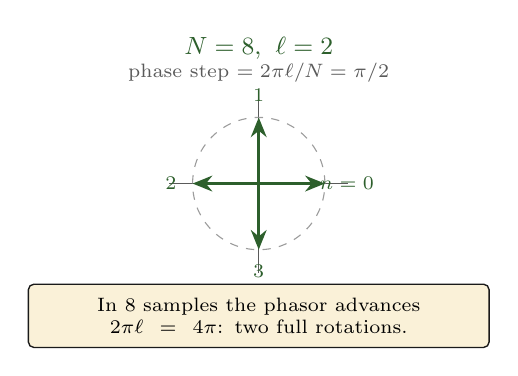
\begin{tikzpicture}[x=0.84cm,y=0.84cm,>=Latex]
      \node[font=\small\bfseries\color{accentgreen}] at (0,2.20) {$N=8,\ \ell=2$};
      \node[font=\scriptsize\color{inkgray}] at (0,1.82) {phase step $=2\pi\ell/N=\pi/2$};
      \draw[inkgray] (-1.35,0.15)--(1.35,0.15);
      \draw[inkgray] (0,-1.20)--(0,1.50);
      \draw[inkgray!60,dashed] (0,0.15) circle (1.0);
      \foreach \ang/\lab in {0/$n=0$,90/$1$,180/$2$,270/$3$} {
        \draw[flowarr,color=accentgreen,line width=1.0pt] (0,0.15)--++(\ang:1.0);
        \node[font=\scriptsize\color{accentgreen}] at ({1.33*cos(\ang)},{0.15+1.33*sin(\ang)}) {\lab};
      }
      \node[notecard,text width=5.5cm,font=\scriptsize] at (0,-1.85) {%
        In $8$ samples the phasor advances $2\pi\ell=4\pi$: two full rotations.};
    \end{tikzpicture}
    \end{center}
  \end{column}
\end{columns}
\takeaway{$e^{\jj2\pi\ell n/N}$ is tone $\ell$ because it rotates at one constant rate and makes exactly $\ell$ turns per OFDM symbol.}
\end{frame}

% =====================================================================
\begin{frame}{What the IFFT transmits}
\storybadge{1}{one tone is a weighted clock}
\small
\begin{columns}[T,onlytextwidth]
  \begin{column}{0.50\textwidth}
    The IFFT builds time samples by adding all tones:
    \[
      x[n]=\frac{1}{N}\sum_{\ell=0}^{N-1}
      d_\ell e^{\jj2\pi \ell n/N}.
    \]
    For a single tone $\ell$:
    \[
      \text{contribution from tone }\ell
      =d_\ell e^{\jj2\pi \ell n/N}.
    \]
    The exponential makes exactly $\ell$ full turns over one OFDM symbol.
  \end{column}
  \begin{column}{0.48\textwidth}
    \begin{center}
    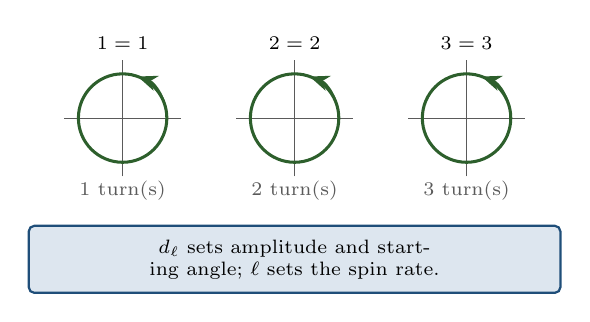
\begin{tikzpicture}[x=0.78cm,y=0.78cm,>=Latex]
      \foreach \ell/\dx in {1/-2.8,2/0,3/2.8} {
        \begin{scope}[shift={(\dx,0.35)}]
          \draw[inkgray] (-0.95,0)--(0.95,0);
          \draw[inkgray] (0,-0.95)--(0,0.95);
          \draw[accentgreen,line width=1.1pt] (0,0) circle (0.72);
          \draw[flowarr,color=accentgreen] (0.72,0) arc (0:70:0.72);
          \node[font=\scriptsize\bfseries] at (0,1.22) {$\ell=\ell$};
          \node[font=\scriptsize\color{inkgray}] at (0,-1.18) {\ell\ turn(s)};
        \end{scope}
      }
      \node[bluecard,text width=6.4cm,font=\scriptsize] at (0,-1.95)
        {$d_\ell$ sets amplitude and starting angle; $\ell$ sets the spin rate.};
    \end{tikzpicture}
    \end{center}
  \end{column}
\end{columns}
\takeaway{OFDM chooses integer-turn clocks on purpose.}
\end{frame}

% =====================================================================
\begin{frame}{What is inside $r[n]$?}
\storybadge{1}{the received sample is a sum of tones}
\small
\begin{columns}[T,onlytextwidth]
  \begin{column}{0.57\textwidth}
    In the clean case, ignore Doppler for a moment. The received sample is the sum of all transmitted tones:
    \[
      r[n]=\sum_{q=0}^{7} d_q e^{\jj2\pi qn/8}+w[n].
    \]
    Written out, the tone $\ell$ is one term inside that sum:
    \[
    \begin{aligned}
      r[n]
      &=d_0e^{\jj2\pi0n/8}
      +d_1e^{\jj2\pi1n/8}
      +\cdots\\
      &\quad+\textcolor{accentred}{d_\ell e^{\jj2\pi\ell n/8}}
      +\cdots
      +d_7e^{\jj2\pi7n/8}
      +w[n].
    \end{aligned}
    \]
    The FFT operation is applied to all of $r[n]$, but linearity lets us follow one highlighted term.
  \end{column}
  \begin{column}{0.40\textwidth}
    \begin{center}
    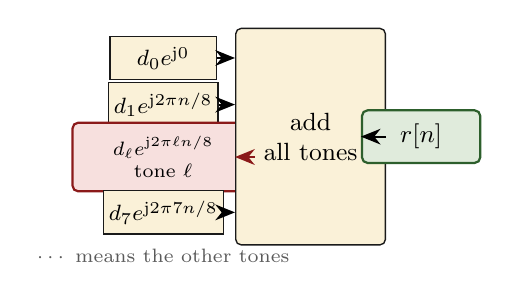
\begin{tikzpicture}[x=0.72cm,y=0.74cm,>=Latex]
      \node[smallbox,minimum width=1.35cm] (d0) at (-1.9,1.55) {$d_0e^{\jj0}$};
      \node[smallbox,minimum width=1.35cm] (d1) at (-1.9,0.75) {$d_1e^{\jj2\pi n/8}$};
      \node[redcard,text width=1.95cm,font=\scriptsize] (dl) at (-1.9,-0.15) {$d_\ell e^{\jj2\pi\ell n/8}$\\tone $\ell$};
      \node[smallbox,minimum width=1.35cm] (d7) at (-1.9,-1.10) {$d_7e^{\jj2\pi7n/8}$};
      \node[notecard,text width=1.55cm,minimum height=2.75cm] (sum) at (0.70,0.20) {add\\all tones};
      \node[greencard,text width=1.15cm] (r) at (2.65,0.20) {$r[n]$};
      \draw[flowarr] (d0)--(sum.west |- d0);
      \draw[flowarr] (d1)--(sum.west |- d1);
      \draw[flowarr,color=accentred,line width=1.0pt] (dl)--(sum.west |- dl);
      \draw[flowarr] (d7)--(sum.west |- d7);
      \draw[flowarr] (sum)--(r);
      \node[font=\scriptsize\color{inkgray},align=center] at (-1.9,-1.85)
        {$\cdots$ means the other tones};
    \end{tikzpicture}
    \end{center}
  \end{column}
\end{columns}
\takeaway{Tone $\ell$ is the highlighted term \(d_\ell e^{\jj2\pi\ell n/8}\) inside the full received sum \(r[n]\).}
\end{frame}

% =====================================================================
\begin{frame}{What FFT bin 4 does}
\storybadge{1}{de-spin first, average second}
\small
\begin{columns}[T,onlytextwidth]
  \begin{column}{0.50\textwidth}
    Bin $4$ asks:
    \begin{center}
      \emph{How much fourth carrier is inside $r[n]$?}
    \end{center}
    It multiplies by the opposite fourth carrier and averages:
    \[
      y_4=\sum_{n=0}^{7} r[n]e^{-\jj2\pi4n/8}.
    \]
    Track the highlighted tone $\ell$ inside $r[n]$. Bin $4$ multiplies that term by $e^{-\jj2\pi4n/8}$:
    \[
      \textcolor{accentred}{d_\ell e^{\jj2\pi\ell n/8}}e^{-\jj2\pi4n/8}
      =
      d_\ell e^{\jj2\pi(\ell-4)n/8}.
    \]
  \end{column}
  \begin{column}{0.48\textwidth}
    \begin{center}
    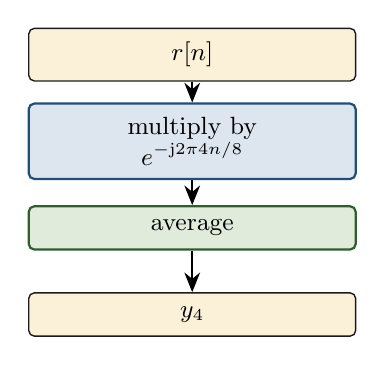
\begin{tikzpicture}[x=1cm,y=1cm,>=Latex]
      \node[notecard,text width=3.8cm] (r) at (0,1.25) {$r[n]$};
      \node[bluecard,text width=3.8cm] (mix) at (0,0.15) {multiply by\\$e^{-\jj2\pi4n/8}$};
      \node[greencard,text width=3.8cm] (avg) at (0,-0.95) {average};
      \node[notecard,text width=3.8cm] (out) at (0,-2.05) {$y_4$};
      \draw[flowarr] (r)--(mix);
      \draw[flowarr] (mix)--(avg);
      \draw[flowarr] (avg)--(out);
    \end{tikzpicture}
    \end{center}
  \end{column}
\end{columns}
\takeaway{An FFT bin is a matched filter: de-spin the carrier you want, then average.}
\end{frame}

% =====================================================================
\begin{frame}{Clean OFDM: bin 4 keeps tone 4}
\storybadge{2}{the wanted tone stops moving}
\small
\begin{columns}[T,onlytextwidth]
  \begin{column}{0.48\textwidth}
    If the incoming tone is $\ell=4$, bin $4$ de-spins it:
    \[
      e^{\jj2\pi4n/8}e^{-\jj2\pi4n/8}=1.
    \]
    So its coefficient is
    \[
      c_{4,4}^{(0)}
      =\frac{1}{8}\sum_{n=0}^{7}1
      =1.
    \]
    The wanted data symbol survives:
    \[
      y_4 \leftarrow 1\cdot d_4.
    \]
  \end{column}
  \begin{column}{0.50\textwidth}
    \begin{center}
    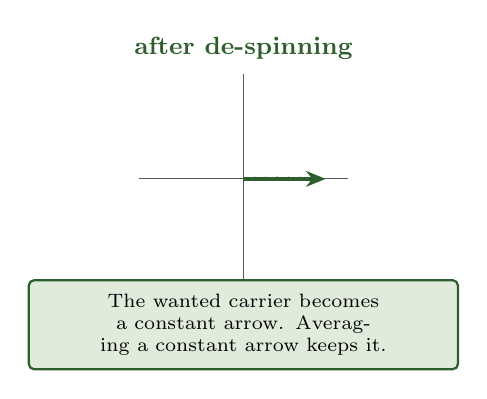
\begin{tikzpicture}[x=0.95cm,y=0.95cm,>=Latex]
      \draw[inkgray] (-1.4,0)--(1.4,0);
      \draw[inkgray] (0,-1.4)--(0,1.4);
      \draw[flowarr,color=accentgreen,line width=1.4pt] (0,0)--(1.1,0);
      \foreach \x in {0.15,0.30,...,1.0} {
        \fill[accentgreen] (\x,0) circle (0.8pt);
      }
      \node[font=\small\bfseries\color{accentgreen}] at (0,1.75) {after de-spinning};
      \node[greencard,text width=5.1cm,font=\scriptsize] at (0,-1.95)
        {The wanted carrier becomes a constant arrow. Averaging a constant arrow keeps it.};
    \end{tikzpicture}
    \end{center}
  \end{column}
\end{columns}
\takeaway{The diagonal coefficient is large because the wanted tone becomes still.}
\end{frame}

% =====================================================================
\begin{frame}{Clean OFDM: bin 4 rejects tone 5}
\storybadge{2}{the neighbour completes one full loop}
\small
\begin{columns}[T,onlytextwidth]
  \begin{column}{0.50\textwidth}
    If the incoming tone is $\ell=5$, bin $4$ sees one leftover turn:
    \[
      e^{\jj2\pi5n/8}e^{-\jj2\pi4n/8}
      =e^{\jj2\pi n/8}.
    \]
    Therefore
    \[
      c_{4,5}^{(0)}
      =\frac{1}{8}\sum_{n=0}^{7}e^{\jj2\pi n/8}=0.
    \]
    The continuous version is the same idea:
    \[
      \int_0^1 e^{\jj2\pi(5-4)t}\,dt=0.
    \]
  \end{column}
  \begin{column}{0.48\textwidth}
    \begin{center}
    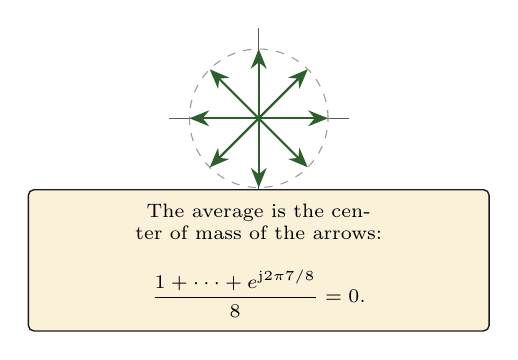
\begin{tikzpicture}[x=0.88cm,y=0.88cm,>=Latex]
      \draw[inkgray] (-1.3,0)--(1.3,0);
      \draw[inkgray] (0,-1.3)--(0,1.3);
      \draw[inkgray!60,dashed] (0,0) circle (1.0);
      \foreach \ang in {0,45,...,315} {
        \draw[flowarr,color=accentgreen,line width=0.8pt] (0,0)--(\ang:1.0);
      }
      \node[notecard,text width=5.5cm,font=\scriptsize] at (0,-2.05)
        {The average is the center of mass of the arrows:
        \[
          \frac{1+\cdots+e^{\jj2\pi7/8}}{8}=0.
        \]};
    \end{tikzpicture}
    \end{center}
  \end{column}
\end{columns}
\takeaway{Clean neighbours cancel because their de-spun loops finish exactly.}
\end{frame}

% =====================================================================
\begin{frame}{A common phase is not ICI}
\storybadge{2}{one useful non-example}
\small
\begin{columns}[T,onlytextwidth]
  \begin{column}{0.50\textwidth}
    A common phase rotates the whole received symbol:
    \[
      r[n]=e^{\jj\phi}x[n].
    \]
    Then
    \[
      y_k=e^{\jj\phi}d_k
    \]
    in clean OFDM. The constellation rotates, but the off-diagonal coefficients stay zero:
    \[
      c_{k,\ell}^{(0)}=0,\qquad \ell\ne k.
    \]
  \end{column}
  \begin{column}{0.48\textwidth}
    \begin{center}
    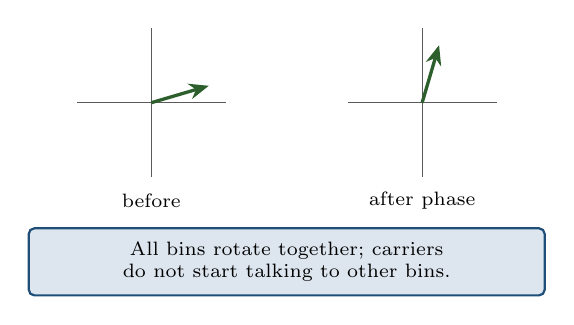
\begin{tikzpicture}[x=0.86cm,y=0.86cm,>=Latex]
      \begin{scope}[shift={(-2.0,0)}]
        \draw[inkgray] (-1.1,0)--(1.1,0);
        \draw[inkgray] (0,-1.1)--(0,1.1);
        \draw[flowarr,color=accentgreen,line width=1.2pt] (0,0)--(0.85,0.25);
        \node[font=\scriptsize] at (0,-1.45) {before};
      \end{scope}
      \begin{scope}[shift={(2.0,0)}]
        \draw[inkgray] (-1.1,0)--(1.1,0);
        \draw[inkgray] (0,-1.1)--(0,1.1);
        \draw[flowarr,color=accentgreen,line width=1.2pt] (0,0)--(0.25,0.85);
        \node[font=\scriptsize] at (0,-1.45) {after phase};
      \end{scope}
      \node[bluecard,text width=6.2cm,font=\scriptsize] at (0,-2.35)
        {All bins rotate together; carriers do not start talking to other bins.};
    \end{tikzpicture}
    \end{center}
  \end{column}
\end{columns}
\takeaway{Common phase is a calibration problem. ICI is a failed cancellation problem.}
\end{frame}

% =====================================================================
\begin{frame}{Doppler changes the spin rates}
\storybadge{3}{the loop no longer lands where it started}
\small
\begin{columns}[T,onlytextwidth]
  \begin{column}{0.50\textwidth}
    Motion time-scales the received waveform. A simple carrier model is
    \[
      f_\ell^{\rx}=(1+a)\ell+\nu.
    \]
    Here:
    \[
      a=\text{wideband scale},\qquad
      \nu=\text{common frequency offset}.
    \]
    Bin $k$ still de-spins by its old grid frequency $k$, so tone $\ell$ has leftover rate
    \[
      \Delta_{k,\ell}=f_\ell^{\rx}-k.
    \]
  \end{column}
  \begin{column}{0.48\textwidth}
    \begin{center}
    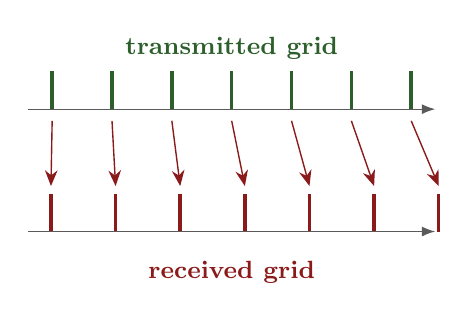
\begin{tikzpicture}[x=0.76cm,y=0.74cm,>=Latex]
      \node[font=\small\bfseries\color{accentgreen}] at (0,2.05) {transmitted grid};
      \foreach \x in {-3,-2,-1,0,1,2,3} {
        \draw[accentgreen,line width=1.25pt] (\x,1.0)--(\x,1.65);
      }
      \draw[inkgray,->] (-3.4,1.0)--(3.4,1.0);
      \node[font=\small\bfseries\color{accentred}] at (0,-1.80) {received grid};
      \foreach \x in {-3,-2,-1,0,1,2,3} {
        \pgfmathsetmacro{\xs}{1.08*\x+0.22}
        \draw[accentred,line width=1.25pt] (\xs,-1.1)--(\xs,-0.45);
        \draw[softarr,color=accentred] (\x,0.8)--(\xs,-0.32);
      }
      \draw[inkgray,->] (-3.4,-1.1)--(3.4,-1.1);
    \end{tikzpicture}
    \end{center}
  \end{column}
\end{columns}
\takeaway{Doppler does not merely rotate a symbol; it changes the relative rates that make FFT cancellation work.}
\end{frame}

% =====================================================================
\begin{frame}{Frequency error becomes phase around the loop}
\storybadge{3}{why $\Delta t$ controls the angle}
\small
\begin{columns}[T,onlytextwidth]
  \begin{column}{0.50\textwidth}
    After bin $k$ de-spins tone $\ell$, the remaining phasor is
    \[
      e^{\jj2\pi\Delta_{k,\ell}t}.
    \]
    Frequency means cycles per symbol, so
    \[
      \Delta_{k,\ell}t
      =
      \text{fraction of a turn at time }t.
    \]
    The coefficient is the time average of that phasor:
    \[
      c_{k,\ell}=\int_0^1 e^{\jj2\pi\Delta_{k,\ell}t}\,dt.
    \]
  \end{column}
  \begin{column}{0.48\textwidth}
    \begin{center}
    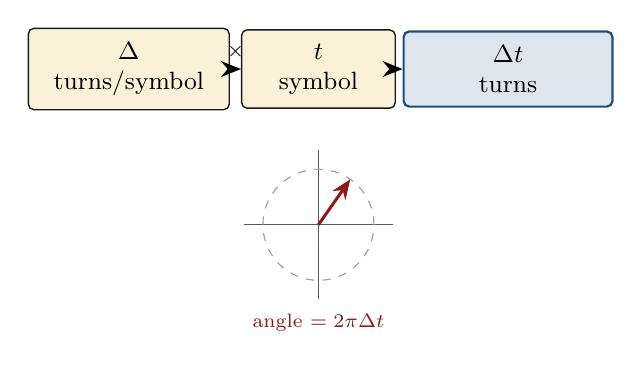
\begin{tikzpicture}[x=0.86cm,y=0.86cm,>=Latex]
      \node[notecard,text width=2.2cm] (rate) at (-2.8,1.15) {$\Delta$\\turns/symbol};
      \node[notecard,text width=1.6cm] (time) at (0.0,1.15) {$t$\\symbol};
      \node[bluecard,text width=2.3cm] (turns) at (2.8,1.15) {$\Delta t$\\turns};
      \draw[flowarr] (rate)--node[above,font=\scriptsize] {$\times$}(time);
      \draw[flowarr] (time)--(turns);
      \begin{scope}[shift={(0,-1.15)}]
        \draw[inkgray] (-1.1,0)--(1.1,0);
        \draw[inkgray] (0,-1.1)--(0,1.1);
        \draw[inkgray!60,dashed] (0,0) circle (0.82);
        \draw[flowarr,color=accentred,line width=1.1pt] (0,0)--(55:0.82);
        \node[font=\scriptsize\color{accentred}] at (0,-1.45)
          {angle $=2\pi\Delta t$};
      \end{scope}
    \end{tikzpicture}
    \end{center}
  \end{column}
\end{columns}
\takeaway{The ICI coefficient is literally the average arrow left by the de-spun carrier.}
\end{frame}

% =====================================================================
\begin{frame}{Doppler makes bin 4 hear tone 5}
\storybadge{3}{the first nonzero off-diagonal term}
\small
\begin{columns}[T,onlytextwidth]
  \begin{column}{0.50\textwidth}
    Use the workbench numbers:
    \[
      k=4,\quad \ell=5,\quad a=0.007,\quad \nu=0.20.
    \]
    The received frequency of tone $5$ is
    \[
      f_5^{\rx}=5(1+0.007)+0.20=5.235.
    \]
    Bin $4$ sees
    \[
      \Delta_{4,5}=5.235-4=1.235.
    \]
    Since $1.235$ is not an integer, the loop misses closure.
  \end{column}
  \begin{column}{0.48\textwidth}
    \[
      c_{4,5}
      =
      \int_0^1 e^{\jj2\pi(1.235)t}\,dt
      \approx 0.128+0.117\jj.
    \]
    \[
      |c_{4,5}|\approx 0.173.
    \]
    \begin{center}
    
\begin{tikzpicture}[x=0.82cm,y=0.82cm,>=Latex]
      \draw[inkgray] (-1.15,0)--(1.15,0);
      \draw[inkgray] (0,-1.15)--(0,1.15);
      \draw[accentred,line width=1.1pt,domain=0:444.6,samples=90]
        plot ({0.88*cos(\x)},{0.88*sin(\x)});
      \draw[flowarr,color=accentred,line width=1.1pt] (0,0)--(0.62,0.38);
      \node[font=\scriptsize\color{accentred}] at (0,-1.45) {leftover average};
    \end{tikzpicture}
    \end{center}
  \end{column}
\end{columns}
\takeaway{Carrier 5 now contributes $c_{4,5}d_5$ inside bin 4. That is ICI.}
\end{frame}

% =====================================================================
\begin{frame}{One coefficient becomes one row term}
\storybadge{3}{the algebra behind the picture}
\small
\begin{columns}[T,onlytextwidth]
  \begin{column}{0.52\textwidth}
    The received waveform contains all carriers:
    \[
      r(t)=\sum_\ell d_\ell e^{\jj2\pi f_\ell^{\rx}t}+n(t).
    \]
    Bin $k$ de-spins and averages:
    \[
      y_k=\int_0^1 r(t)e^{-\jj2\pi kt}\,dt.
    \]
    Substitute the sum:
    \[
      y_k=\sum_\ell d_\ell
      \underbrace{\int_0^1 e^{\jj2\pi(f_\ell^{\rx}-k)t}\,dt}_{c_{k,\ell}}
      +n_k.
    \]
  \end{column}
  \begin{column}{0.46\textwidth}
    \begin{center}
    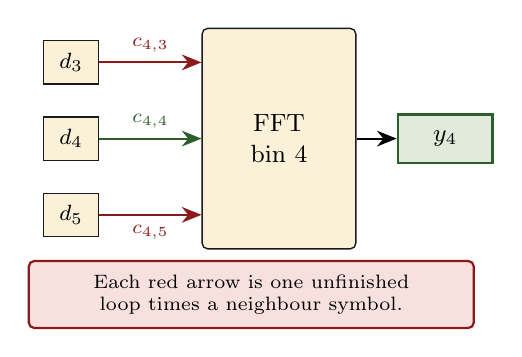
\begin{tikzpicture}[x=0.88cm,y=0.88cm,>=Latex]
      \node[smallbox] (d3) at (-2.4,1.1) {$d_3$};
      \node[smallbox] (d4) at (-2.4,0.0) {$d_4$};
      \node[smallbox] (d5) at (-2.4,-1.1) {$d_5$};
      \node[notecard,text width=1.6cm,minimum height=2.8cm] (bin) at (0.6,0) {FFT\\bin 4};
      \node[method,minimum width=1.2cm] (y) at (3.0,0) {$y_4$};
      \draw[flowarr,color=accentred] (d3)--node[above,font=\scriptsize] {$c_{4,3}$}(bin.west |- d3);
      \draw[flowarr,color=accentgreen] (d4)--node[above,font=\scriptsize] {$c_{4,4}$}(bin.west);
      \draw[flowarr,color=accentred] (d5)--node[below,font=\scriptsize] {$c_{4,5}$}(bin.west |- d5);
      \draw[flowarr] (bin)--(y);
      \node[redcard,text width=5.3cm,font=\scriptsize] at (0.2,-2.25)
        {Each red arrow is one unfinished loop times a neighbour symbol.};
    \end{tikzpicture}
    \end{center}
  \end{column}
\end{columns}
\takeaway{The ICI matrix is just all the loop averages collected into rows.}
\end{frame}

% =====================================================================
\begin{frame}{The row sum is why one-tap equalization struggles}
\storybadge{3}{the unknown neighbours remain}
\small
\begin{columns}[T,onlytextwidth]
  \begin{column}{0.48\textwidth}
    Clean OFDM:
    \[
      y_k=c_{k,k}d_k+n_k,\qquad c_{k,\ell}=0\quad(\ell\ne k).
    \]
    With Doppler:
    \[
      y_k=c_{k,k}d_k+
      \sum_{\ell\ne k}c_{k,\ell}d_\ell+n_k.
    \]
    One-tap equalization can divide by $c_{k,k}$, but it cannot know the unknown neighbour symbols $d_\ell$.
  \end{column}
  \begin{column}{0.50\textwidth}
    \begin{center}
    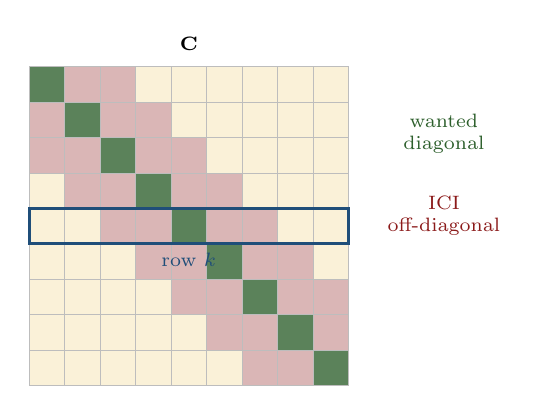
\begin{tikzpicture}[x=0.45cm,y=0.45cm]
      \foreach \r in {0,...,8} {
        \foreach \c in {0,...,8} {
          \pgfmathtruncatemacro{\dist}{abs(\r-\c)}
          \ifnum\dist=0
            \fill[accentgreen!78] (\c,8-\r) rectangle ++(1,1);
          \else
            \ifnum\dist<3
              \fill[accentred!32] (\c,8-\r) rectangle ++(1,1);
            \else
              \fill[paper] (\c,8-\r) rectangle ++(1,1);
            \fi
          \fi
          \draw[inkgray!40,line width=0.2pt] (\c,8-\r) rectangle ++(1,1);
        }
      }
      \draw[accentblue,line width=1.2pt] (0,4) rectangle (9,5);
      \node[font=\scriptsize\bfseries] at (4.5,9.65) {$\mathbf C$};
      \node[font=\scriptsize\color{accentblue}] at (4.5,3.55) {row $k$};
      \node[font=\scriptsize\color{accentgreen},align=center] at (11.7,7.1) {wanted\\diagonal};
      \node[font=\scriptsize\color{accentred},align=center] at (11.7,4.8) {ICI\\off-diagonal};
    \end{tikzpicture}
    \end{center}
  \end{column}
\end{columns}
\takeaway{Doppler turns independent bins into a coupled linear system.}
\end{frame}

% =====================================================================
\begin{frame}{Why one full FFT is fragile}
\storybadge{4}{it averages before you can use time structure}
\small
\begin{columns}[T,onlytextwidth]
  \begin{column}{0.50\textwidth}
    A full FFT bin produces one scalar:
    \[
      y_k^{\mathrm{full}}
      =\int_0^1 r(t)e^{-\jj2\pi kt}\,dt.
    \]
    That scalar is already the final average. It no longer remembers how the desired arrow and the leakage arrow moved during the symbol.

    \medskip
    \textbf{Problem:} Doppler is a time-evolution effect, but the full FFT stores one end result.
  \end{column}
  \begin{column}{0.48\textwidth}
    \begin{center}
    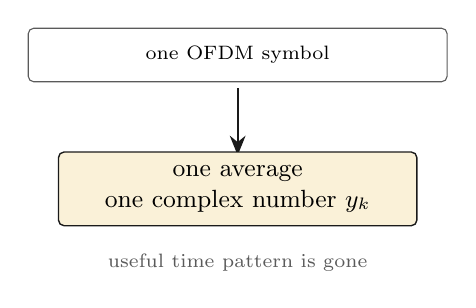
\begin{tikzpicture}[x=0.95cm,y=0.85cm,>=Latex]
      \draw[inkgray,rounded corners=2pt] (-2.8,0.55) rectangle (2.8,1.35);
      \node[font=\scriptsize] at (0,0.95) {one OFDM symbol};
      \draw[flowarr,color=ink] (0,0.45)--(0,-0.55);
      \node[notecard,text width=4.2cm] at (0,-1.05) {one average\\one complex number $y_k$};
      \node[font=\scriptsize\color{inkgray},align=center] at (0,-2.15)
        {useful time pattern is gone};
    \end{tikzpicture}
    \end{center}
  \end{column}
\end{columns}
\takeaway{The problem is not that averaging is wrong; it is that the receiver averages too early.}
\end{frame}

% =====================================================================
\begin{frame}{Partial FFT keeps short-time views}
\storybadge{4}{split before the final average}
\small
\begin{columns}[T,onlytextwidth]
  \begin{column}{0.50\textwidth}
    Split the symbol into $M$ windows. In each window, run the same bin-$k$ de-spin and local average:
    \[
      z_{m,k}
      =
      M\int_{m/M}^{(m+1)/M}
      r(t)e^{-\jj2\pi kt}\,dt.
    \]
    Now bin $k$ has a vector:
    \[
      \mathbf z_k=[z_{0,k},z_{1,k},\ldots,z_{M-1,k}]^T.
    \]
  \end{column}
  \begin{column}{0.48\textwidth}
    \begin{center}
    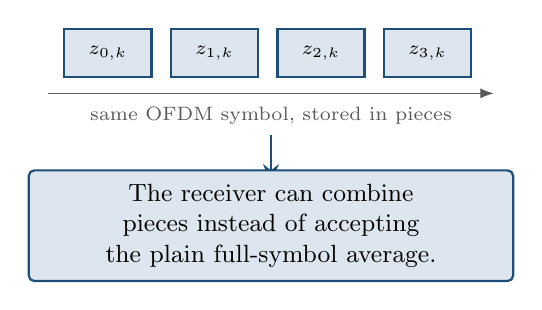
\begin{tikzpicture}[x=0.82cm,y=0.82cm,>=Latex]
      \foreach \m in {0,...,3} {
        \draw[draw=accentblue,fill=blubg,line width=0.8pt] (-3.2+\m*1.65,0.8) rectangle ++(1.35,0.75);
        \node[font=\scriptsize] at (-2.525+\m*1.65,1.17) {$z_{\m,k}$};
      }
      \draw[inkgray,->] (-3.45,0.55)--(3.45,0.55);
      \node[font=\scriptsize\color{inkgray}] at (0,0.20) {same OFDM symbol, stored in pieces};
      \draw[flowarr,color=accentblue] (0,-0.10)--(0,-0.85);
      \node[bluecard,text width=5.8cm] at (0,-1.50)
        {The receiver can combine pieces instead of accepting the plain full-symbol average.};
    \end{tikzpicture}
    \end{center}
  \end{column}
\end{columns}
\takeaway{Partial FFT changes the observation from one scalar into a branch vector.}
\end{frame}

% =====================================================================
\begin{frame}{What the weights are trying to do}
\storybadge{4}{align wanted, scramble unwanted}
\small
\begin{columns}[T,onlytextwidth]
  \begin{column}{0.50\textwidth}
    The receiver forms
    \[
      \widetilde y_k=\frac{1}{M}\sum_{m=0}^{M-1}w_{m,k}z_{m,k}.
    \]
    The same weights have two jobs:
    \[
      \text{desired:}\quad
      \frac{1}{M}\sum_m w_{m,k}c^{(m)}_{k,k}\approx 1,
    \]
    \[
      \text{leakage:}\quad
      \frac{1}{M}\sum_m w_{m,k}c^{(m)}_{k,\ell}\approx 0.
    \]
  \end{column}
  \begin{column}{0.48\textwidth}
    \begin{center}
    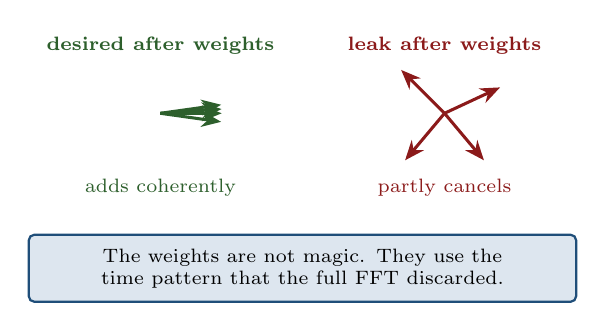
\begin{tikzpicture}[x=0.82cm,y=0.82cm,>=Latex]
      \node[font=\scriptsize\bfseries\color{accentgreen}] at (-2.2,2.0) {desired after weights};
      \foreach \a in {0,8,-8,4} {
        \draw[flowarr,color=accentgreen,line width=1.1pt] (-2.2,0.95)--++(\a:0.95);
      }
      \node[font=\scriptsize\color{accentgreen}] at (-2.2,-0.20) {adds coherently};

      \node[font=\scriptsize\bfseries\color{accentred}] at (2.2,2.0) {leak after weights};
      \foreach \a in {25,135,230,310} {
        \draw[flowarr,color=accentred,line width=1.1pt] (2.2,0.95)--++(\a:0.95);
      }
      \node[font=\scriptsize\color{accentred}] at (2.2,-0.20) {partly cancels};

      \node[bluecard,text width=6.6cm,font=\scriptsize] at (0,-1.45)
        {The weights are not magic. They use the time pattern that the full FFT discarded.};
    \end{tikzpicture}
    \end{center}
  \end{column}
\end{columns}
\takeaway{Partial FFT works because desired and leakage evolve differently across short windows.}
\end{frame}

% =====================================================================
\begin{frame}{A tiny before/after number}
\storybadge{4}{same example, less leakage}
\small
\begin{columns}[T,onlytextwidth]
  \begin{column}{0.45\textwidth}
    For the same $k=4,\ell=5$ example:
    \[
      \left|\frac{c_{4,5}}{c_{4,4}}\right|
      \approx 0.189
      \qquad\text{(full FFT)}.
    \]
    With $M=4$ partial FFT branches and weights chosen for bin $4$:
    \[
      \left|\frac{\widetilde c_{4,5}}{\widetilde c_{4,4}}\right|
      \approx 0.0066.
    \]
    That is about $29$ dB less selected leakage.
  \end{column}
  \begin{column}{0.53\textwidth}
    \begin{center}
    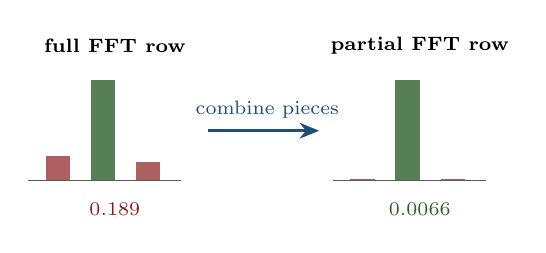
\begin{tikzpicture}[x=0.88cm,y=0.88cm,>=Latex]
      \node[font=\scriptsize\bfseries] at (-2.2,1.95) {full FFT row};
      \fill[accentred!70] (-3.2,0) rectangle ++(0.35,0.35);
      \fill[accentgreen!80] (-2.55,0) rectangle ++(0.35,1.45);
      \fill[accentred!70] (-1.90,0) rectangle ++(0.35,0.27);
      \draw[inkgray] (-3.45,0)--(-1.25,0);
      \node[font=\scriptsize\color{accentred}] at (-2.2,-0.42) {$0.189$};

      \node[font=\scriptsize\bfseries] at (2.2,1.95) {partial FFT row};
      \fill[accentred!70] (1.2,0) rectangle ++(0.35,0.03);
      \fill[accentgreen!80] (1.85,0) rectangle ++(0.35,1.45);
      \fill[accentred!70] (2.50,0) rectangle ++(0.35,0.02);
      \draw[inkgray] (0.95,0)--(3.15,0);
      \node[font=\scriptsize\color{accentgreen}] at (2.2,-0.42) {$0.0066$};

      \draw[flowarr,color=accentblue,line width=1.0pt] (-0.85,0.72)--(0.75,0.72);
      \node[font=\scriptsize\color{accentblue}] at (0,1.02) {combine pieces};
    \end{tikzpicture}
    \end{center}
  \end{column}
\end{columns}
\takeaway{The desired bin stays loud; the selected off-diagonal term gets much quieter.}
\end{frame}

% =====================================================================
\begin{frame}{Where RPC and JUNA fit}
\storybadge{4}{same physics, different weight learning}
\small
\begin{columns}[T,onlytextwidth]
  \begin{column}{0.48\textwidth}
    Partial FFT creates the branch vector $\mathbf z_k$. The receiver still needs good weights $\mathbf w_k$.
    \vspace{0.20cm}

    RPC:
    \[
      \text{pilots}\longrightarrow \mathbf w_k.
    \]
    JUNA:
    \[
      \text{pilots + reliable LDPC feedback}\longrightarrow \mathbf w_k.
    \]
  \end{column}
  \begin{column}{0.50\textwidth}
    \begin{center}
    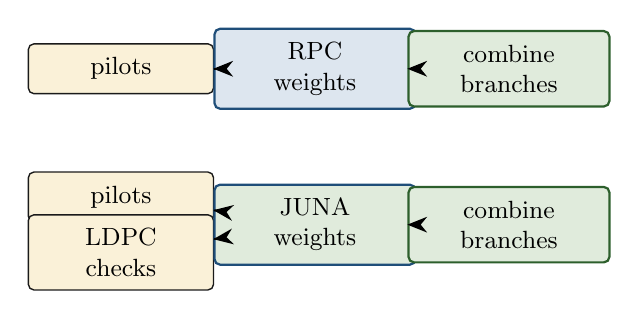
\begin{tikzpicture}[x=0.88cm,y=0.88cm,>=Latex]
      \node[notecard,text width=2.0cm] (p1) at (-2.6,1.0) {pilots};
      \node[bluecard,text width=2.2cm] (rpc) at (0.2,1.0) {RPC\\weights};
      \node[greencard,text width=2.2cm] (o1) at (3.0,1.0) {combine\\branches};
      \draw[flowarr] (p1)--(rpc);
      \draw[flowarr] (rpc)--(o1);

      \node[notecard,text width=2.0cm] (p2) at (-2.6,-0.85) {pilots};
      \node[notecard,text width=2.0cm] (ldpc) at (-2.6,-1.65) {LDPC\\checks};
      \node[bluecard,text width=2.2cm,fill=grnbg] (juna) at (0.2,-1.25) {JUNA\\weights};
      \node[greencard,text width=2.2cm] (o2) at (3.0,-1.25) {combine\\branches};
      \draw[flowarr] (p2)--(juna);
      \draw[flowarr] (ldpc)--(juna);
      \draw[flowarr] (juna)--(o2);
    \end{tikzpicture}
    \end{center}
  \end{column}
\end{columns}
\takeaway{RPC and JUNA differ in how they learn weights; the partial-FFT mitigation mechanism is the same.}
\end{frame}

% =====================================================================
\begin{frame}{One-sentence mental model}
\storybadge{$\star$}{what a new grad student should leave with}
\small
\begin{center}
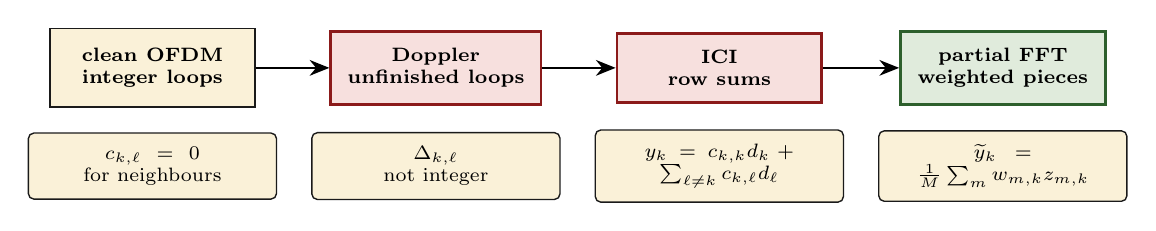
\begin{tikzpicture}[x=1cm,y=0.86cm,>=Latex]
  \node[flowbox,minimum width=2.6cm,font=\scriptsize\bfseries] (a) at (-5.4,1.1) {clean OFDM\\integer loops};
  \node[issue,minimum width=2.6cm,font=\scriptsize\bfseries] (b) at (-1.8,1.1) {Doppler\\unfinished loops};
  \node[issue,minimum width=2.6cm,font=\scriptsize\bfseries] (c) at (1.8,1.1) {ICI\\row sums};
  \node[method,minimum width=2.6cm,font=\scriptsize\bfseries] (d) at (5.4,1.1) {partial FFT\\weighted pieces};
  \draw[flowarr] (a)--(b);
  \draw[flowarr] (b)--(c);
  \draw[flowarr] (c)--(d);

  \node[notecard,text width=2.8cm,font=\scriptsize] at (-5.4,-0.35) {$c_{k,\ell}=0$\\for neighbours};
  \node[notecard,text width=2.8cm,font=\scriptsize] at (-1.8,-0.35) {$\Delta_{k,\ell}$\\not integer};
  \node[notecard,text width=2.8cm,font=\scriptsize] at (1.8,-0.35) {$y_k=c_{k,k}d_k+\sum_{\ell\ne k}c_{k,\ell}d_\ell$};
  \node[notecard,text width=2.8cm,font=\scriptsize] at (5.4,-0.35) {$\widetilde y_k=\frac1M\sum_m w_{m,k}z_{m,k}$};
\end{tikzpicture}
\end{center}
\vspace{0.1cm}
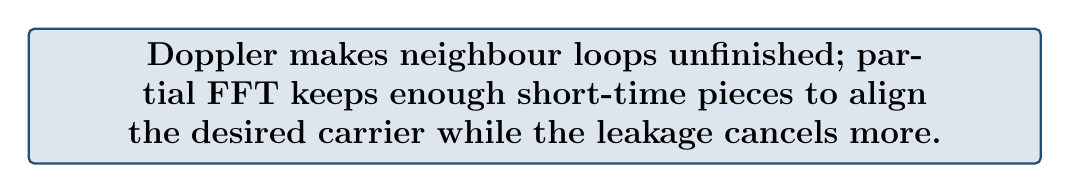
\begin{tikzpicture}
  \node[bluecard,text width=12.5cm,font=\large] {%
    \textbf{Doppler makes neighbour loops unfinished; partial FFT keeps enough short-time pieces to align the desired carrier while the leakage cancels more.}};
\end{tikzpicture}
\end{frame}

\end{document}
